% Adapted from Alex Reustle's CMSC351 Course Notes

% This program is free software: you can redistribute it and/or modify
% it under the terms of the GNU General Public License as published by
% the Free Software Foundation, either version 3 of the License, or
% (at your option) any later version.

% This program is distributed in the hope that it will be useful,
% but WITHOUT ANY WARRANTY; without even the implied warranty of
% MERCHANTABILITY or FITNESS FOR A PARTICULAR PURPOSE.  See the
% GNU General Public License for more details.

% You should have received a copy of the GNU General Public License
% along with this program.  If not, see <http://www.gnu.org/licenses/>.
\documentclass[english, 10pt]{article}

\usepackage{notes}
\usepackage{gensymb}
\usepackage{inconsolata}
\usepackage[shellescape]{gmp}
\allowdisplaybreaks%
\newcommand{\thiscoursecode}{CMSC 320}
\newcommand{\thiscoursename}{Introduction to Data Science}
\newcommand{\thisprof}{Prof.\ John Dickerson}
\newcommand{\me}{Akilesh Praveen}
\newcommand{\thisterm}{Fall 2020}
\newcommand{\website}{https://cmsc320.github.io}%chktex 8
\usepackage{ifpdf}
\ifpdf%
\DeclareGraphicsRule{*}{mps}{*}{}
\fi
% \listfiles

\usepackage[utf8]{inputenc}
 
\usepackage{listings}
\usepackage{xcolor}
\usetikzlibrary{patterns}
\usepackage[many]{tcolorbox}
 
\definecolor{codegreen}{rgb}{0,0.6,0}
\definecolor{codegray}{rgb}{0.5,0.5,0.5}
\definecolor{codepurple}{rgb}{0.58,0,0.82}
\definecolor{backcolour}{rgb}{0.95,0.95,0.94}
\definecolor{codered}{rgb}{0.5,0.15,0.15}
\definecolor{commentred}{rgb}{1,0.01,0.02}
 
\lstdefinestyle{mystyle}{
    backgroundcolor=\color{backcolour},   
    commentstyle=\color{codegreen},
    keywordstyle=\color{red},
    numberstyle=\tiny\color{codegray},
    stringstyle=\color{codered},
    basicstyle=\ttfamily\footnotesize,
    breakatwhitespace=false,         
    breaklines=true,                 
    captionpos=b,                    
    keepspaces=true,
    xleftmargin=.15\textwidth,
    xrightmargin=.15\textwidth,
    linewidth=\textwidth,                 
    numbers=left,                    
    numbersep=5pt,                  
    showspaces=false,                
    showstringspaces=false,
    showtabs=false,                  
    tabsize=2,
    belowskip=3em,
    aboveskip=3em,
}

\lstset{style=mystyle}


% \VerbEnvir{align tikzpicture algorithm}
%%%Headers
\chead{320 - Intro to Data Science}
\lhead{\thisterm}

%%%%% TITLE %%%%%
\graphicspath{{../}}
\newcommand{\notefront}{%
\pagenumbering{arabic}
\begin{center}
{\small}
\textbf{\Huge{\noun{\thiscoursecode}}}
{\Huge \par}
{\Large{\noun{\thiscoursename}}}\\
\vspace{0.1in}
\vspace{0in}\includegraphics[scale=0.3]{umd_cs.jpg} \\
\vspace{0.1in}{\noun\me} \\
{\noun\thisprof} \ $\bullet$ \ {\noun\thisterm} \ $\bullet$ \ {\noun{University of Maryland}} \\
{\ttfamily \url{\website}} \\
\end{center}
}

 \tikzstyle{class}=[
    rectangle,
    draw=black,
    text centered,
    anchor=north,
    text=black,
    text width=2cm,
    shading=axis,
    bottom color={rgb:red,222;green,222;blue,222},
    top color=white,shading angle=45]

\begin{document}
% \renewcommand\familydefault{\sfdefault}
% \sffamily
  % Notes front
  \notefront%
  % Table of Contents and List of Figures
  \tocandfigures%
  
\section{Notes \& Preface}

Course notes for CMSC320, under Prof. John Dickerson. Notes collected from previous and current lectures.

\section{Lecture 1}

\subsection{What is Data Science?}

Data Science is the application of computation and statistical techniques to address or gain insight.
It's the intersection of statistics and Computer Science.
Based on what I've learned thus far, learning to do data science is like learning how to use a TI-84 in statistics class.
You're simply learning how to leverage programming tools in order to perform advanced, complex, and meaningful data-related operations.\newline

It's the use of statistics and computer science in order to find real-world insights.\newline\newline

{
\centering


\tikzset{every picture/.style={line width=0.75pt}} %set default line width to 0.75pt        

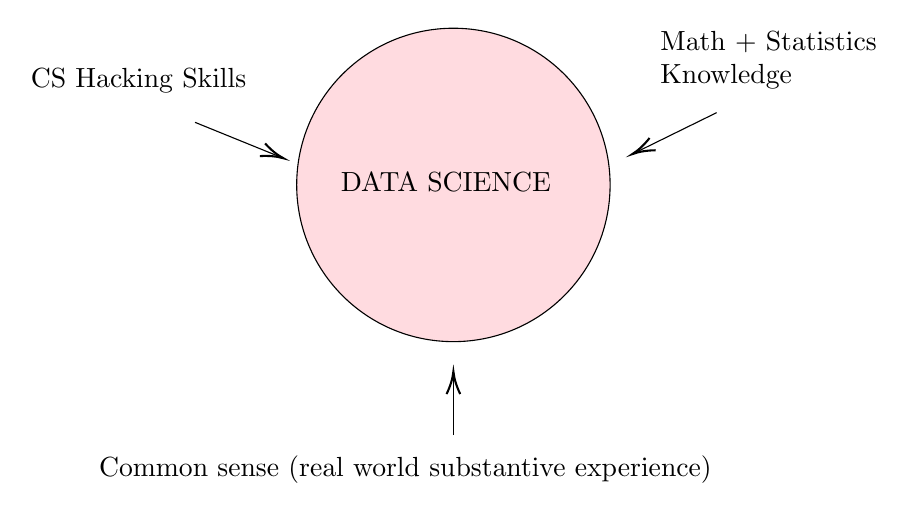
\begin{tikzpicture}[x=0.75pt,y=0.75pt,yscale=-1,xscale=1]
%uncomment if require: \path (0,300); %set diagram left start at 0, and has height of 300

%Shape: Circle [id:dp061140258122834745] 
\draw  [fill={rgb, 255:red, 255; green, 219; blue, 224 }  ,fill opacity=1 ] (254.67,119.5) .. controls (254.67,77.8) and (288.47,44) .. (330.17,44) .. controls (371.86,44) and (405.67,77.8) .. (405.67,119.5) .. controls (405.67,161.2) and (371.86,195) .. (330.17,195) .. controls (288.47,195) and (254.67,161.2) .. (254.67,119.5) -- cycle ;
%Straight Lines [id:da4450208385410075] 
\draw    (205.67,89.33) -- (246.48,105.91) ;
\draw [shift={(248.33,106.67)}, rotate = 202.11] [color={rgb, 255:red, 0; green, 0; blue, 0 }  ][line width=0.75]    (10.93,-3.29) .. controls (6.95,-1.4) and (3.31,-0.3) .. (0,0) .. controls (3.31,0.3) and (6.95,1.4) .. (10.93,3.29)   ;
%Straight Lines [id:da055339322100053545] 
\draw    (457,84.67) -- (418.13,103.78) ;
\draw [shift={(416.33,104.67)}, rotate = 333.81] [color={rgb, 255:red, 0; green, 0; blue, 0 }  ][line width=0.75]    (10.93,-3.29) .. controls (6.95,-1.4) and (3.31,-0.3) .. (0,0) .. controls (3.31,0.3) and (6.95,1.4) .. (10.93,3.29)   ;
%Straight Lines [id:da5012858238681945] 
\draw    (330.17,240) -- (330.17,211.33) ;
\draw [shift={(330.17,209.33)}, rotate = 450] [color={rgb, 255:red, 0; green, 0; blue, 0 }  ][line width=0.75]    (10.93,-3.29) .. controls (6.95,-1.4) and (3.31,-0.3) .. (0,0) .. controls (3.31,0.3) and (6.95,1.4) .. (10.93,3.29)   ;

% Text Node
\draw (274.67,112.5) node [anchor=north west][inner sep=0.75pt]   [align=left] {DATA SCIENCE};
% Text Node
\draw (125.33,62) node [anchor=north west][inner sep=0.75pt]   [align=left] {CS Hacking Skills};
% Text Node
\draw (428.67,44.33) node [anchor=north west][inner sep=0.75pt]   [align=left] {Math + Statistics\\Knowledge};
% Text Node
\draw (158.17,248.67) node [anchor=north west][inner sep=0.75pt]   [align=left] {Common sense (real world substantive experience)};


\end{tikzpicture}

}

\subsection{Topics}

Here are the general topics that this class will cover.

\begin{itemize}
	\item Processing data
	\item Visualizing data
	\item Understanding data
	\item Communicating data
	\item Extracting value from data
\end{itemize}

\subsection{Tools}

Here are some tools commonly employed by data scientists. We'll try to cover how to use most of them here.

\begin{itemize}
	\item Python
	\item Scikit-Learn
	\item Docker
	\item PANDAS
	\item Spark
	\item TensorFlow
\end{itemize}

\subsection{Conda}

Conda is a package and environment manager for python that we can use with the command line.
We can create multiple environments for us and install separate packages in each of them.
This will be highly useful to us, as we sometimes want to consolidate the tools we use into separate environments.

\section{Lecture 2}

\begin{tcolorbox}[title=Definition:,colframe=red!75!black,colback=red!5!white,arc=0pt,fonttitle=\bfseries]
\textbf{Data Collection} $\rightarrow$ The process of measuring and gathering information on targeted variables.
\end{tcolorbox}

\subsection{Literate Programming}

The idea of \textbf{literate programming} is that you have the source code, an explanation of the source code, and the end result of running the code all in one file. Usually, this file is identified as a \textit{notebook}. In other words, the syntax is no different from regular code, you just get a more organized way to show off tables, plots, and other outputs generated from your code.

\subsection{Jupyter Notebook + Alternatives}

Jupyter Notebook is a service that started off as \texttt{iPython}, but it's basically a web-based platform that we use for literate programming. Specifically, it supports Python-based literate programming. Most data scientists prefer it, and it can also apparently leverage big data tools, such as Apache Spark.\newline

It saves files in \texttt{.ipynb} format, which most platforms (i.e. GitHub) have built in viewers for. Options to export in other readable formats are available. Basically, it's just Python with a bunch of bells and whistles on top to make the output of your code look pretty.\newline

\textit{Apache Zeppelin} is an alternative data analysis tool, but we will stick to Jupyter for our purposes. This is because Jupyter seems to be preferred in industry.\newline

\textit{RStudio} is the equivalent, for people who prefer to use the \texttt{R} programming language for data science.\newline

This course will be centered around Jupyter Notebook.

\subsection{List Comprehensions in Python}

To make lists in Python, you can use loops or the \texttt{map()} function, but a \textit{pythonic} way of doing this would be to use a list comprehension. Below is a simple example.\newline

\begin{tcolorbox}
\textbf{Example:} Make a list of all the squares of \texttt{\{0,1,2,3,4,5,6,7,8,9\}}\newline\newline
\textbf{List Comprehension:}\newline
\texttt{squares = [i * i for i in range(10)]}
\end{tcolorbox}

A good way of thinking about this is that it allows you to build sets like a mathematician. This is a common theme in data science, where we can find the intersection between a lot of math stuff and computer science stuff. It's good to know how lists are generated in a mathematical sense in Python for that reason. Here's an example where we translate mathematical notation into a Python list comprehension.\\

\begin{tcolorbox}
\textbf{Example:} Make a list of all odd natural numbers from 0 to 999\\\\
\textbf{Math Notation:}\\ $E =$ \{$x$ | $x$ in $\mathbb{N} \land x$ is odd $\land x<1000$ \}\\\\
\textbf{List Comprehension:}\\
\texttt{E = [x for x in range(1000) if x \% 2 != 0]}
\end{tcolorbox}

\subsection{Using Python3}

We will use Python3. Since I used Python2 during my internship, I'm going to note some big changes to keep track of.\\

\begin{itemize}
	\item Python3 is backwards incompatible. (Don't write in Python2!)
	\item Print has changed from a command to a function, so make sure to use proper function notation when invoking it.
	\item Division has changed. \texttt{1/2} no longer equals 0. \texttt{1/2 == 0.5} and floored division is now taken care of this way: \texttt{1//2 == 0}
\end{itemize}

\subsection{Python vs. R for Data Scientists}

Some arguments for both sides in terms of what to use.

\begin{itemize}
	\item Python is a 'full' programming langauge. Also, if you've got prior experience with Python paradigms or just programming in general, that's a big plus in terms of learning curve.
	\item R has more mature 'pure statistics' libraries, but Python is apparently catching up.
	\item In terms of \textbf{processing speed}, R is certainly faster. It was designed and optimized for statistics processing.
	\item Python is preferable for machine learning operations, which is pretty big right now.
\end{itemize}

My personal choice will be to use Python as much as I can when I'm studying this course. Since it's more prominent in the tech industry, I should be using it more anyway.

\subsection{The Classic Statistical View of Data}

There are \textbf{four} main types of data: Nominal, Ordinal, Interval, and Ratio data. They can each be classified under two main subgroups, Categorical and Numerical data. Here's a visualization.\\

{
\centering



\tikzset{every picture/.style={line width=0.75pt}} %set default line width to 0.75pt        

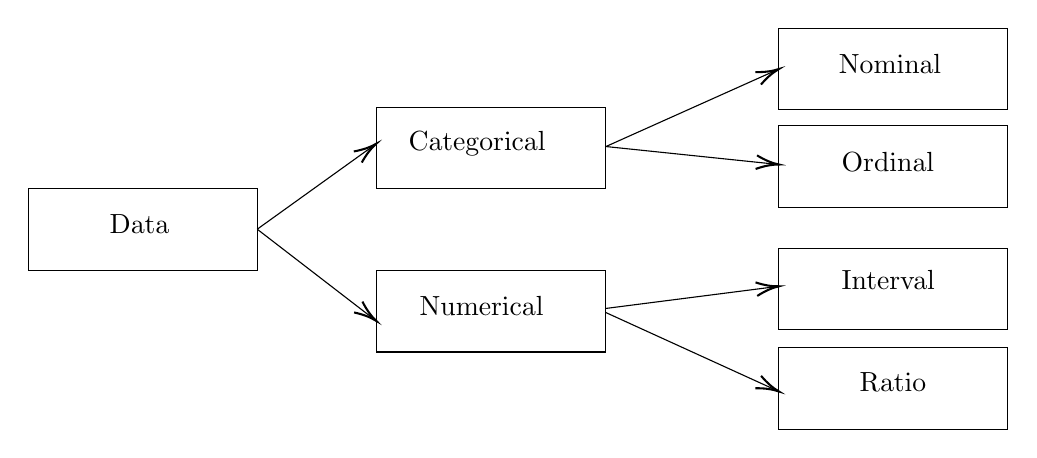
\begin{tikzpicture}[x=0.75pt,y=0.75pt,yscale=-1,xscale=1]
%uncomment if require: \path (0,300); %set diagram left start at 0, and has height of 300

%Shape: Rectangle [id:dp8149613399348021] 
\draw   (72,131) -- (182.33,131) -- (182.33,170.33) -- (72,170.33) -- cycle ;
%Shape: Rectangle [id:dp680618887900226] 
\draw   (239.67,91.67) -- (350,91.67) -- (350,131) -- (239.67,131) -- cycle ;
%Shape: Rectangle [id:dp777477779359951] 
\draw   (239.67,170.33) -- (350,170.33) -- (350,209.67) -- (239.67,209.67) -- cycle ;
%Shape: Rectangle [id:dp9580214955547155] 
\draw   (433.67,53.67) -- (544,53.67) -- (544,93) -- (433.67,93) -- cycle ;
%Shape: Rectangle [id:dp19525566557447283] 
\draw   (433.67,100.5) -- (544,100.5) -- (544,139.83) -- (433.67,139.83) -- cycle ;
%Shape: Rectangle [id:dp18958725273981114] 
\draw   (433.67,159.67) -- (544,159.67) -- (544,199) -- (433.67,199) -- cycle ;
%Shape: Rectangle [id:dp27616820331988945] 
\draw   (433.67,207.67) -- (544,207.67) -- (544,247) -- (433.67,247) -- cycle ;
%Straight Lines [id:da07504069427898741] 
\draw    (182.33,150.5) -- (238.04,110.5) ;
\draw [shift={(239.67,109.33)}, rotate = 504.32] [color={rgb, 255:red, 0; green, 0; blue, 0 }  ][line width=0.75]    (10.93,-3.29) .. controls (6.95,-1.4) and (3.31,-0.3) .. (0,0) .. controls (3.31,0.3) and (6.95,1.4) .. (10.93,3.29)   ;
%Straight Lines [id:da18494381831895634] 
\draw    (182.33,150.5) -- (238.08,193.45) ;
\draw [shift={(239.67,194.67)}, rotate = 217.61] [color={rgb, 255:red, 0; green, 0; blue, 0 }  ][line width=0.75]    (10.93,-3.29) .. controls (6.95,-1.4) and (3.31,-0.3) .. (0,0) .. controls (3.31,0.3) and (6.95,1.4) .. (10.93,3.29)   ;
%Straight Lines [id:da49166239871511697] 
\draw    (350.33,110.67) -- (431.84,74.15) ;
\draw [shift={(433.67,73.33)}, rotate = 515.87] [color={rgb, 255:red, 0; green, 0; blue, 0 }  ][line width=0.75]    (10.93,-3.29) .. controls (6.95,-1.4) and (3.31,-0.3) .. (0,0) .. controls (3.31,0.3) and (6.95,1.4) .. (10.93,3.29)   ;
%Straight Lines [id:da6935259459415319] 
\draw    (350.33,110.67) -- (431.68,119.13) ;
\draw [shift={(433.67,119.33)}, rotate = 185.94] [color={rgb, 255:red, 0; green, 0; blue, 0 }  ][line width=0.75]    (10.93,-3.29) .. controls (6.95,-1.4) and (3.31,-0.3) .. (0,0) .. controls (3.31,0.3) and (6.95,1.4) .. (10.93,3.29)   ;
%Straight Lines [id:da6050313931467277] 
\draw    (350.33,190.67) -- (431.85,227.84) ;
\draw [shift={(433.67,228.67)}, rotate = 204.51] [color={rgb, 255:red, 0; green, 0; blue, 0 }  ][line width=0.75]    (10.93,-3.29) .. controls (6.95,-1.4) and (3.31,-0.3) .. (0,0) .. controls (3.31,0.3) and (6.95,1.4) .. (10.93,3.29)   ;
%Straight Lines [id:da8985137963347964] 
\draw    (350.33,188.67) -- (431.68,178.25) ;
\draw [shift={(433.67,178)}, rotate = 532.71] [color={rgb, 255:red, 0; green, 0; blue, 0 }  ][line width=0.75]    (10.93,-3.29) .. controls (6.95,-1.4) and (3.31,-0.3) .. (0,0) .. controls (3.31,0.3) and (6.95,1.4) .. (10.93,3.29)   ;

% Text Node
\draw (110,142.17) node [anchor=north west][inner sep=0.75pt]   [align=left] {Data};
% Text Node
\draw (254,102) node [anchor=north west][inner sep=0.75pt]   [align=left] {Categorical};
% Text Node
\draw (259.33,181.33) node [anchor=north west][inner sep=0.75pt]   [align=left] {Numerical};
% Text Node
\draw (461.33,65) node [anchor=north west][inner sep=0.75pt]   [align=left] {Nominal};
% Text Node
\draw (462.67,112) node [anchor=north west][inner sep=0.75pt]   [align=left] {Ordinal};
% Text Node
\draw (462.67,168.83) node [anchor=north west][inner sep=0.75pt]   [align=left] {Interval};
% Text Node
\draw (471.33,218.33) node [anchor=north west][inner sep=0.75pt]   [align=left] {Ratio};


\end{tikzpicture} \\
}

\subsubsection{Nominal Data}

A type of categorical data, nominal data value have names and describe the state of things. For example, your marriage status is nominal data because you can either be \textit{single}, \textit{married}, or \textit{separated}. Another example is the type of drink you're going to have. Will it be \textit{Milk}, \textit{Beer}, or \textit{Juice}?\\

The key here is that there can be no quantitative values assigned to each of these categories, as that would allow us to do math with them and would defeat the purpose of these labels. These values \textbf{cannot be easily compared}, so they have no material value. \textit{E.g. being single is not quantitatively better than being married (objectively), and vice versa}.\\

\begin{tcolorbox}
\textbf{Example:} What is your marital status?
\begin{itemize}
	\item Married
	\item Divorced (separated)
	\item Single
\end{itemize}
\end{tcolorbox}

\subsubsection{Ordinal Data}

Ordinal data represents values that have names that describe the state of things, but in this case, there \textbf{is} an ordering of those values. This is what sets it apart from nominal data. \\ 
\begin{tcolorbox}
\textbf{Example:} What did you think of the movie?
\begin{itemize}
	\item Strongly liked
	\item Liked
	\item Indifferent
	\item Disliked
	\item Strongly Disliked
\end{itemize}
\end{tcolorbox}

Given how subjective some of these things can be, the distinction between nominal and ordinal can be \textbf{blurry} at times. For example, going back to our nominal example, some people may think that being single is quantitatively better than being married.

\subsubsection{Interval and Ratio Data}

Interval and Ratio data are pretty similar, and both can be used to measure things that can be represented by either integers or real numbers. \\

\textbf{Interval} data scales with fixed but arbitrary values. That might sound silly, but a good example is \textbf{dates}. Below is an example of two data comparisons of interval data that seem arbitrary, but indeed hold integer value.\\

\begin{tcolorbox}
\textbf{Example:} The following two operations are equal. \\\\
\texttt{10/1/2019 - 9/1/2019} \\
\texttt{10/1/2018 - 9/1/2018}
\end{tcolorbox}

The measures don't look like integer values at first, but we can quantify them by marking them with days.\\

Here's what sets \textbf{Interval} data apart, however. You have \textbf{no method} of computing ratios or scales with it. For example, never mind that you can try computing \texttt{(9/1/2019 $\times$ 8/25/2015)}, the unit of the answer would be totally useless to us, and neither would the actual number, even if you went ahead with the operation.\\

\textbf{Ratio} data is, in essence, the same as interval data in that it is numerical, but the scale itself \textbf{has a true zero}. While dates don't necessarily have a true zero, we can say that money counts as ratio data. For example, having zero money means that you're at the absolute zero of that scale, whereas the absolute zero for dates is disputable. Are we saying we're starting at O A.D.? The Big Bang? Even earlier?\\

Differentiating between the two is usually a case-by-case basis thing, which is what I'm thinking is the best way to handle any conflicts I end up running into between ratio and interval data.\\

\begin{tcolorbox}
\textbf{Example:} Interval data \\\\
Temperature on the scale of Celsius or Fahrenheit is interval-type data because $0\degree$ is set to an arbitrarily fixed point. Also, we can't scale it properly- $30\degree F$ isn't twice as hot as $15\degree F$.
\end{tcolorbox}

\begin{tcolorbox}
\textbf{Example:} Ratio data \\\\
Temperature on the Kelvin scale is ratio data. $0K$ is set at legitimate absolute zero, and $50K$ is truly twice as cold as $100K$.
\end{tcolorbox}

\subsection{Data Science at a Glance}








\section{Test Section}

\subsection{Lower Level}

Here's a cool code example.

{\centering
\begin{lstlisting}[language=C]
#include <stdio.h>
#include <math.h>

int main() {
   double value;

   printf("Enter a number: ");
   scanf("%lf", &value);     /* Notice the use of %lf */

   printf("sqrt %f: \n", sqrt(value));
   printf("power of 2: %f\n", pow(value, 2));
   printf("sin: %f\n", sin(value));

   return 0;
}
\end{lstlisting}
}

Here's some more information about our code example.



\section{Footnotes}

Taken by Akilesh Praveen.

\end{document}
